%%%%%%%%%%%%%%%%%%%%%%%%%%%%%%%%%%%%%%%%%
% Beamer Presentation
% LaTeX Template
% Version 1.0 (10/11/12)
%
% This template has been downloaded from:
% http://www.LaTeXTemplates.com
%
% License:
% CC BY-NC-SA 3.0 (http://creativecommons.org/licenses/by-nc-sa/3.0/)
%
%%%%%%%%%%%%%%%%%%%%%%%%%%%%%%%%%%%%%%%%%

%----------------------------------------------------------------------------------------
%	PACKAGES AND THEMES
%----------------------------------------------------------------------------------------

\documentclass{beamer}

\mode<presentation> {

% The Beamer class comes with a number of default slide themes
% which change the colors and layouts of slides. Below this is a list
% of all the themes, uncomment each in turn to see what they look like.

%\usetheme{default}
%\usetheme{AnnArbor}
%\usetheme{Antibes}
%\usetheme{Bergen}
%\usetheme{Berkeley}
%\usetheme{Berlin}
%\usetheme{Boadilla}
%\usetheme{CambridgeUS}
%\usetheme{Copenhagen}
%\usetheme{Darmstadt}
%\usetheme{Dresden}
%\usetheme{Frankfurt}
%\usetheme{Goettingen}
%\usetheme{Hannover}
%\usetheme{Ilmenau}
%\usetheme{JuanLesPins}
%\usetheme{Luebeck}
\usetheme{Madrid}
%\usetheme{Malmoe}
%\usetheme{Marburg}
%\usetheme{Montpellier}
%\usetheme{PaloAlto}
%\usetheme{Pittsburgh}
%\usetheme{Rochester}
%\usetheme{Singapore}
%\usetheme{Szeged}
%\usetheme{Warsaw}

% As well as themes, the Beamer class has a number of color themes
% for any slide theme. Uncomment each of these in turn to see how it
% changes the colors of your current slide theme.

%\usecolortheme{albatross}
%\usecolortheme{beaver}
%\usecolortheme{beetle}
%\usecolortheme{crane}
%\usecolortheme{dolphin}
%\usecolortheme{dove}
%\usecolortheme{fly}
%\usecolortheme{lily}
%\usecolortheme{orchid}
%\usecolortheme{rose}
%\usecolortheme{seagull}
%\usecolortheme{seahorse}
%\usecolortheme{whale}
%\usecolortheme{wolverine}

%\setbeamertemplate{footline} % To remove the footer line in all slides uncomment this line
%\setbeamertemplate{footline}[page number] % To replace the footer line in all slides with a simple slide count uncomment this line

%\setbeamertemplate{navigation symbols}{} % To remove the navigation symbols from the bottom of all slides uncomment this line
}

\usepackage{graphicx} % Allows including images
\usepackage{booktabs} % Allows the use of \toprule, \midrule and \bottomrule in tables
\usepackage{listings}
\usepackage{amsmath}
\usepackage{algorithm,algorithmic}
\usepackage{graphicx}

%----------------------------------------------------------------------------------------
%	TITLE PAGE
%----------------------------------------------------------------------------------------

\title[L\'ogica Epist\'emica]{L\'ogica Epist\'emica} % The short title appears at the bottom of every slide, the full title is only on the title page

\author{Andr\'es Laurito} % Your name
\institute[L\'ogicas Modales] % Your institution as it will appear on the bottom of every slide, may be shorthand to save space
{
Primer cuatrimestre 2016 \\ % Your institution for the title page
\medskip
\textit{andy.laurito@hotmail.com} % Your email address
}
\date{\today} % Date, can be changed to a custom date

\begin{document}

\begin{frame}
\titlepage % Print the title page as the first slide
\end{frame}

\begin{frame}
\frametitle{Lo que vamos a ver} % Table of contents slide, comment this block out to remove it
\tableofcontents % Throughout your presentation, if you choose to use \section{} and \subsection{} commands, these will automatically be printed on this slide as an overview of your presentation
\end{frame}

%----------------------------------------------------------------------------------------
%	PRESENTATION SLIDES
%----------------------------------------------------------------------------------------

%------------------------------------------------
\section{Introducci\'on al problema} 
%------------------------------------------------

\subsection{Los papers}

\begin{frame}
\frametitle{¿Qu\'e papers eleg\'i para presentar?}
\begin{enumerate}
\item On the Complexity of Epistemic Reasoning
\item Which Semantics for Neighbourhood Semantics?
\end{enumerate}

\begin{block}{Idea de hac\'ia donde vamos}
Tratan el problema de la l\'ogica epist\'emica. En el primero nos vamos a enfocar en la complejidad computacional de SAT para la l\'ogica epist\'emica, mientras que en el otro vamos a usar est\'e estudio, para definir la complejidad computacional de la bisimulaci\'on en 2 modelos sem\'anticos de Neighbourhood.
\end{block}


\end{frame}

\subsection{L\'ogica epist\'emica}

\begin{frame}
\frametitle{¿Qu\'e es la l\'ogica epist\'emica?}
\begin{block}{Wikipedia}
La l\'ogica epist\'emica es un campo de la l\'ogica modal que se ocupa del razonamiento sobre el conocimiento. Est\'a tiene aplicaciones en numerosos campos, tales como filosof\'ia, ciencia computacional te\'orica, inteligencia artificial, econom\'ia y lingu\'istica.
\end{block}

\begin{block}{Stanford Enciclopedy of Phylosophy}
Epistemic logic is the logic of knowledge and belief. It provides insight into the properties of individual knowers, has provided a means to model complicated scenarios involving groups of knowers and has improved our understanding of the dynamics of inquiry. 
\end{block}

\end{frame}

\begin{frame}
\frametitle{¿Qu\'e es la l\'ogica epist\'emica?}
\begin{block}{Mi definici\'on}
Es la l\'ogica de la representaci\'on del conocimiento y las creencias de un individuo (en I.A. un agente). 
A partir de la extensi\'on de la l\'ogica proposicional con operadores modales, podemos modelar de manera formal el poseer conocimientos y adquirirlos (en donde adquirir puede ser visto como una forma de razonamiento del individuo).
\end{block}

Super relacionada con Belief Revision (me parece bastante vol\'atil el fin de una y el comienzo de otra).
\end{frame}

\section{El problema - Parte 1}

\subsection{Definiendo la sem\'antica}

\begin{frame}
\frametitle{Introduciendo a los nuevos operadores}
En las l\'ogicas epist\'emicas existen dos operadores modales. Si a representa un agente, escribimos:
\begin{itemize}
\item a conoce una f\'ormula $\phi$ como $K_{a}\phi$ 
\item a cree una f\'ormula $\phi$ como $B_{a}\phi$ 
\end{itemize}

Para el problema que vamos a atacar, es indistinto el operador. En todo lo que sigue de la presentaci\'on , voy a usar el primer operador y lo voy a notar con la notaci\'on utilizada en toda la materia, pero debe etenderser que es indistinto usar cualquiera de los dos. \\~\\

Queremos modelar a la epistemolog\'ia, tenemos la sintaxis,\\
los operadores ... ¿Qu\'e modelo sem\'antico usamos?
\end{frame}

%------------------------------------------------

\begin{frame}
\frametitle{Usando el modelo de Kripke}
Nos encontramos con un problema conocido como el "logical omniscience problem". Sabemos que: 
\begin{block}{Lema}
Si $\phi$ y ($\phi \implies \psi$) son v\'alidas en un modelo, tambi\'en lo es $\psi$.
\end{block}

Y recordando que K tiene la regla de necesitaci\'on que dice:
\begin{block}{Necesitaci\'on}
Si $\phi$ es v\'alida en un modelo, entonces tambi\'en lo es $\Box\phi$ .
\end{block}
Llegamos a que la l\'ogica modal K es muy fuerte para modelar conocimiento y creencia!.
\end{frame}

%------------------------------------------------

\begin{frame}
\frametitle{Neighbourhood al rescate!}
Vamos a definir a una estructura epist\'emica, (los famosos modelos de vecindad con otro sabor), como una tripla $M = (W,N,I)$ en donde, si A es un conjunto de agentes, y a $\in$ A entonces: \\~\\
\begin{itemize}
\item $W$ es un conjunto de mundos
\item $N: A x W \mapsto 2^{2^{W}}$ es la funci\'on que asigna a cada agente en un mundo, el correspondiente conjunto de proposiciones que conoce (es decir, un conjunto epist\'emico).
\item $I: P \mapsto 2^{W}$ es la funci\'on que asigna a cada proposici\'on at\'omica, el conjunto de mundos en donde dicha proposici\'on es satisfecha.
\end{itemize}

La definici\'on de satisfacibilidad de una f\'ormula ser\'a la misma que vimos en la materia.
\end{frame}

\begin{frame}
\frametitle{Problema con Neighbourhood}

Si bien con el modelo definido reci\'en, solucionamos el problema de logical omniscience, nos surge un nuevo problema. Citando la diapo 6 de la tecera clase: 

\begin{block}{Teorema}
Si $\phi \iff \psi$ es v\'alida en una clase de modelos de vecindad, entonces en dicha clase tambi\'en lo es $\Box\phi \iff \Box\psi$ .
\end{block} 

Nos vamos a permitir vivir con este problema

\end{frame}

\subsection{Modelando la noci\'on de poder de razonamiento}
\begin{frame}
\frametitle{El razonamiento como f\'ormulas}
\begin{enumerate}
\item $\neg \Box false$
\item $\Box true$
\item $\Box(p \land q)\implies \Box q$
\item $(\Box p \land \Box q)\implies \Box (p \land q)$
\item $\Box p \implies \Box\Box p$
\item $\neg \Box p \implies \Box \neg \Box p$
\item $\Box p \implies p$
\end{enumerate}
\end{frame}

\begin{frame}
\frametitle{El razonamiento modelado sobre conjuntos epist\'emicos!}
\begin{enumerate}
\item $\emptyset \notin N(a,w)$
\item $W \in N(a,w)$
\item Si $U \in N(a,w)$ y $U \subseteq V, \implies V \in N(a,w)$
\item Si $U \in N(a,w)$ y $V \in N(a,w) \implies (U \cap V) \in N(a,w)$
\item Si $U \in N(a,w) \implies \{u : U \in N(a,u)\} \in N(a,w)$
\item Si $U \notin N(a,w) \implies \{u : U \notin N(a,u)\} \in N(a,w)$
\item Si $U \in N(a,w) \implies w \in U$
\end{enumerate}

A partir de est\'a definici\'on, si llamamos $\epsilon$ a la clase de todos los modelos epist\'emicos, entonces podemos decir:

\begin{block}{Definici\'on}
Sea S un subconjunto de $\{1,...,7\}$, entonces $\epsilon_{S}$ ser\'a la clase de los modelos epist\'emicos que satisfaga $C_{j}$ $\forall j \in S$
\end{block} 
\end{frame}

\subsection{Estudiando la complejidad computacional}

\begin{frame}
\frametitle{Complejidad computacional de cada modelo ?}

Sabemos que una f\'ormula $\phi$ es $\epsilon_{S}$-satisfacible si $\exists w \in W$ tal que $\epsilon_{S} \models_{w} \phi$. C\'ual ser\'a la relaci\'on, si es que la hay, entre S y la complejidad computacional de satisfacer una f\'ormula?
\end{frame}

\begin{frame}
\frametitle{EL problema a resolver en este paper}

\begin{block}{EL Teorema}
 Si S es un subconjunto de {1, ..., 7} entonces resolver SAT est\'a en PSPACE. Ahora, si S es un subconjunto de {1, ..., 7} y $4 \notin S$, entonces SAT est\'a en NP
\end{block}

El paper de "On the Complexity of Epistemic Reasoning" demuestra este teorema (todo el paper est\'a enfocado en esto).
\end{frame}

\begin{frame}
\frametitle{La idea para resolver el problema}

El objetivo para demostrar el teorema anterior viene por este lado

\begin{block}{La idea}
Sea M uno de los modelos epist\'emicos $\epsilon_{i}$ con $i \in S$, $\phi$ una f\'ormula tal que $\epsilon_{i} \models \phi$. La idea ser\'a probar que siempre que $i \neq 4$ existe una valuaci\'on v para $\phi$ tal que las subformul\'as con operadores modales en $\phi$ son satisfacibles, si $\psi$ es satisfacible, con $\psi$ una f\'ormula perteneciente al calc\'ulo proposicional.
\end{block}

Con esto podemos aplicar el algoritmo de tableau de una manera m\'as eficiente. Adem\'as, al dar propiedades de est\'a pinta, nos podemos construir un algoritmo no determin\'istico de tiempo polinomial.

Veamos la propiedad enunciada m\'as importante del paper:
\end{frame}

\begin{frame}
\frametitle{SAT de una f\'ormula}

\begin{block}{Proposici\'on 1}
Una f\'ormula $\phi$ es $\epsilon$-satisfacible $iff \exists$ v valuaci\'on para $\phi$ tal que si $\Box\psi_{1}$ y $\Box \psi_{2} \in sub(\phi), v(\Box \psi_{1}) = 1$, y $v(\Box\psi_{2}) = 0 \implies (\psi_{1} \land \psi_{2}) \lor (\neg \psi_{1} \land \psi_{2})$ es $\epsilon$-satisfacible
\end{block}

A partir de est\'a propiedad, podemos inferir el siguiente algoritmo:

\begin{block}{Algoritmo SAT para $\epsilon$}
\begin{itemize}
	\item De manera no determinist\'isca adivinar una valuaci\'on v para $\phi$
	\item $\forall \Box\psi_{1} \land \Box\psi_{2} \in sub(\phi)$ / $v(\Box\psi_{1}) = 1 \land v(\Box\psi_{2}) = 0$ no determin\'isticamente y de manera recursiva, verificar que $(\psi_{1} \land \neg\psi_{2})$ \'o $(\neg\psi_{1}\land\psi_{2})$ es satisfacible.
\end{itemize}
\end{block}

Estamos recortando un monton de ramas del algoritmo de Tableau !!. (Otra propiedad muy importante que enuncia el paper)

\end{frame}

\begin{frame}
\frametitle{Propiedas sobre los modelos de razonamiento}

A partir de la proposici\'on 1, podemos dar propiedades sobre cada $\epsilon_{i}$, y obtener el algoritmo de manera similar a como lo hicimos reci\'en. Veamos algunos ejemplos:

\begin{block}{Proposici\'on 2}
Una f\'ormula $\phi$ es $\epsilon_{2}$-satisfacible $iff \exists$ v valuaci\'on para $\phi$ tal que: 
\begin{itemize}
\item Si $\Box\psi \in sub(\phi)$ y  $v(\Box \psi) = 0 \implies \neg \psi$ es $\epsilon_{2}-$satisfacible, y 
\item $\Box\psi_{1}$ y $\Box \psi_{2} \in sub(\phi), v(\Box \psi_{1}) = 1$, y $v(\Box \psi_{2}) = 0 \implies (\psi_{1} \land \psi_{2}) \lor (\neg \psi_{1} \land \psi_{2})$ es $\epsilon_{2}$-satisfacible
\end{itemize}
\end{block}

\begin{block}{Proposici\'on 3}
Una f\'ormula $\phi$ es $\epsilon_{3}$-satisfacible $iff \exists$ v valuaci\'on para $\phi$ tal que: 
\begin{itemize}
\item $\Box\psi_{1}$ y $\Box \psi_{2} \in sub(\phi), v(\Box \psi_{1}) = 1$, y $v(\Box \psi_{2}) = 0 \implies (\psi_{1} \land \neg\psi_{2})$ es $\epsilon_{3}$-satisfacible
\end{itemize}
\end{block}
\end{frame}

\begin{frame}
\frametitle{Un momento...}

Antes hab\'ia mencionado que si el agente pod\'ia razonar:
Si $U \in N(a,w)$ y $V \in N(a,w) \implies (U \cap V) \in N(a,w)$ (poder inferir conocimiento), el problema de SAT se volv\'ia PSPACE.
¿Por qu\'e pasa esto?

\begin{block}{Lema}
Sea $M = (W,N,I) \in \epsilon_{4}$, sea $\phi$ una f\'ormula y $w \in W$. Entonces $M \nvDash_{w}\Box\phi \iff \cap_{j = 1}^{k} U_{j} \neq I(\phi)$ para todo subconjunto no vac\'io ${U_{1},...,U_{k}} \subseteq N(a,w)$  
\end{block}

Y entonces la propiedad que caracteriza a $\epsilon_{4}$ es la siguiente:

\begin{block}{Proposici\'on 4}
Una f\'ormula $\phi$ es $\epsilon_{4}$-satisfacible $iff \exists$ v valuaci\'on para $\phi$ tal que: 
\begin{itemize}
\item $\Box\psi_{1}, ..., \Box\psi_{k} \in sub(\phi), v(\Box \psi_{j}) = 1$ $\forall 1 \leq j \le k \land v(\Box\psi_{k}) = 0$ $\implies \land_{j = 1}^{k-1} \psi_{j} \land \neg\psi_{k}$ es $\epsilon_{4}$-satisfacible \'o $\neg\psi_{j}\land\psi_{k}$ es $\epsilon_{4}$-satisfacible para alg\'un j, $1 \leq j \le k$
\end{itemize}
\end{block}
\end{frame}

\section{El problema - Parte 2}

\subsection{Redefiniendo la sem\'antica}
\begin{frame}
\frametitle{Repasando lo que tenemos}

En toda est\'a primera parte, al igual que en la materia, decimos que:

\begin{block}{Definici\'on}
 Sea M un modelo epist\'emico, $w \in W$, $M\models_{w} \Box\phi \iff \{v / v\models \phi\} \in N(a,w)$. 
\end{block}
Vamos a decir lo mismo de otra forma:

\begin{block}{Reescribiendo la definici\'on}
 Sea M un modelo epist\'emico, $w \in W$, $M\models_{w} \Box\phi \iff \{v / v\models \phi\} \in N(a,w)=\{X_{1}, ...,X_{n}\} \iff \exists Y \in N(a,w) / Y = \{v / v\models \phi\} \iff \exists Y \in N(a,w) / Y = ||\phi||_{M}$
\end{block}

Esto puede leerse como : Un agente a cree una f\'ormula $\phi$, desde un estado o mundo w $\iff$ el conjunto de TODOS los mundos en donde $\phi$ es cierta pertenece a N(a,w)... No ser\'a mucho pedir todos?

\end{frame}

\begin{frame}
\frametitle{Nuevo enfoque}

Cambio la notaci\'on por una cuesti\'on de practicidad. Vamos a representar al operador modal que conocemos, el $\Box$ como $[]$, y vamos a definir una nueva sem\'antica.

\begin{block}{Sem\'antica fuerte}
Vamos a decir que $||[=]\phi||_{M} = \{w | \exists X \in N(a,w)$ tal que $X = ||\phi||_{M}\}$
\end{block}


\begin{block}{Sem\'antica debil}
Vamos a decir que $||[\subseteq]\phi||_{M} = \{w | \exists X \in N(a,w)$ tal que $X \subseteq ||\phi||_{M}\}$
\end{block}

Estas sem\'anticas son conocidas hoy en d\'ia para la l\'ogica epist\'emica, e incluso ambas poseen una noci\'on de bisimulaci\'on. El objetivo del segundo paper, "Which Semantics for Neighbourhood Semantics?", tratar\'a el problema de definir un nuevo concepto de bisimulaci\'on para la primer sem\'antica, y mostrar\'a la complejidad computacional usando fuertemente las propiedades vistas del primer paper. 
\end{frame}

\subsection{Bisimulaci\'on en la sem\'antica de Neighbourhood}

\begin{frame}
\frametitle{Definiendo bisimulaci\'on}

\begin{block}{$N_{\subseteq}$-bisimulaci\'on}
Sean M y $M^{'}$ dos modelos epist\'emicos. Una $N_{\subseteq}$-bisimulaci\'on entre M y $M^{'}$ es una relaci\'on no vac\'ia $Z \subseteq$ $WxW^{'}$ tal que si $xZx^{'}$ entonces:
\begin{itemize}
\item Prop: $\forall p \in PROP$, $x \in ||p|||_{M} \iff x^{'} \in ||p||_{M^{'}}$
\item Zig: $\forall T \in N_{x}$, $\exists T^{'} \in N^{'}_{x} tal que \forall w^{'} \in T^{'} \exists w \in T$ tal que $wZw^{'}$
\item Zag: $\forall T^{'} \in N^{'}_{x}$, $\exists T \in N_{x} tal que \forall w \in T \exists w^{'} \in T^{'}$ tal que $wZw^{'}$
\end{itemize}
\end{block}

Es muy parecida a la noci\'on de bisimulaci\'on que vimos en la materia. Veamos ahora como definimos la noci\'on de bisimulaci\'on para la otra sem\'antica.

\end{frame}

\begin{frame}
\frametitle{Definiendo bisimulaci\'on}

\begin{block}{$N_{=}$-bisimulaci\'on}
Sean M y $M^{'}$ dos modelos epist\'emicos. Una $N_{=}$-bisimulaci\'on entre M y $M^{'}$ es una relaci\'on no vac\'ia $Z \subseteq$ $WxW^{'}$ tal que si $xZx^{'}$ entonces:
\begin{itemize}
\item Prop: $\forall p \in PROP$, $x \in ||p|||_{M} \iff x^{'} \in ||p||_{M^{'}}$
\item Zig: $\forall T \in N_{x}$, $\exists T^{'} \in N^{'}_{x}$ tal que 
\begin{itemize}
\item $\forall w^{'} \in T^{'} \exists w \in T$ tal que $wZw^{'}$
\item $\forall w^{'} \in W^{'}\backslash T^{'} \exists w \in W\backslash T$ tal que $wZw^{'}$
\end{itemize}
\item Zig: $\forall T^{'} \in N_{x}^{'}$, $\exists T \in N_{x}$ tal que 
\begin{itemize}
\item $\forall w \in T$ $\exists w^{'} \in T^{'}$ tal que $wZw^{'}$
\item $\forall w \in W\backslash T$ $\exists w^{'} \in W^{'}\backslash T^{'}$ tal que $wZw^{'}$
\end{itemize}  
\end{itemize}
\end{block}

El problema con est\'a definici\'on es que es muy fuerte. La bisimulaci\'on preserva satisfacibilidad de las f\'ormulas de $N_{=}$, pero l\'imita el poder de expresividad de $N_{=}$

\end{frame}

\begin{frame}
\frametitle{Redefiniendo $N_{=}$-bisimulaci\'on}

\begin{block}{Definici\'on de diferenciaci\'on}
Se define la clase de modelos epist\'emicos diferenciales D como 
D = $\{M | \forall w \in W$ $\forall T \in N_{w}$ $\exists \phi$ tal que $||\phi^{M}|| = T\}$
\end{block}
Lo importante es notar que para cada conjunto de mundos en la vecindad, existe una f\'ormula que caracteriza a dicho conjunto.

A partir de est\'a definici\'on, podemos volver a definir el concepto de $N_{=}$-bisimulaci\'on como sigue

\end{frame}

\begin{frame}
\frametitle{Redefiniendo $N_{=}$-bisimulaci\'on}

\begin{block}{$N_{=}$-bisimulaci\'on}
Sean M y $M^{'}$ dos modelos epist\'emicos. Una $N_{\subseteq}$-bisimulaci\'on entre M y $M^{'}$ es una relaci\'on no vac\'ia $Z \subseteq$ $WxW^{'}$ tal que si $xZx^{'}$ entonces:
\begin{itemize}
\item Prop: $\forall p \in PROP$, $x \in ||p|||_{M} \iff x^{'} \in ||p||_{M^{'}}$
\item Zig: $\forall T \in N_{x}$, $\exists T^{'} \in N^{'}_{x}$ tal que 
\begin{itemize}
\item $\forall w^{'} \in T^{'} \exists w \in T$ tal que $wZw^{'}$
\item $\forall X^{'} \notin N^{'}_{w^{'}}$ diferenciable en $M^{'}$ tal que $T^{'} \subset X^{'} \subseteq W^{'}$, existen $w^{'} \in X^{'} \backslash T^{'}$, $w \in W\backslash T$ tal que $wZw^{'}$
\end{itemize}
\item Zig: $\forall T^{'} \in N_{x}^{'}$, $\exists T \in N_{x}$ tal que 
\begin{itemize}
\item $\forall w \in T$ $\exists w^{'} \in T^{'}$ tal que $wZw^{'}$
\item $\forall X \notin N_{w}$ diferenciable en $M$ tal que $T \subset X \subseteq W$, existen $w \in X \backslash T$, $w^{'} \in W^{'}\backslash T^{'}$ tal que $wZw^{'}$
\end{itemize}  
\end{itemize}
\end{block}

Por que pasa que la definici\'on se vuelve tan complicada ?.

\end{frame}

\begin{frame}
\frametitle{Extendiendo a $N_{=}$}

El aporte importante que hace el paper, es resolver a la pregunta anterior. Definimos al operador $\bigtriangledown$ como sigue:

\begin{block}{Definici\'on nuevo operador $\bigtriangledown$}
$||\phi \bigtriangledown \psi||^{M} = \{w | \exists X_{1}, X_{2} \in N_{w}$ tal que $X_{1} \neq X_{2} \land X_{1} = ||\phi||_{M} \land X_{2} = ||\phi \lor \psi||_{M}\}$
\end{block}

Con este operador, podemos probar que que la l\'ogica $N_{=}(\bigtriangledown)$ (es la l\'ogica que obtenemos al extender $N_{=}$ con el operador $\bigtriangledown$), matchea el poder expresivo de las $N_{=}$-bisimulaciones.

El problema con este nuevo operador, es que es alto galerazo. No habr\'a algo m\'as natural?
\end{frame}

\begin{frame}
\frametitle{El operador modal de existencia}

Definimos al operador modal de existencia E como sigue:

\begin{block}{Definici\'on operador modal de existencia}
\[ ||E\phi|| = \begin{cases} 
      W & si ||\phi||_{M} \neq \emptyset \\
      \emptyset & sino
   \end{cases}
\]
\end{block}

Se puede probar que vale la siguiente igualdad
$||\phi \bigtriangledown \psi||^{M} = ||[=]\phi \land [=](\phi \lor \psi) \land E(\psi \land \neg \phi)||^{M}$

Por lo que a partir de esto, podemos inferir que la extensi\'on $N_{=}(E)$ matchea el poder expresivo de las $N_{=}$-bisimulaciones.

Surge la siguiente pregunta... Habremos modificado la complejidad computacional, al haber extendido de est\'a manera la bisimulaci\'on?
\end{frame}
%------------------------------------------------

\subsection{Estudiando la complejidad computacional}

\begin{frame}
\frametitle {Satisfacibilidad de las sem\'anticas definidas}

\begin{block}{Proposici\'on}
$\forall \phi$ y $\forall$ M modelo epist\'emico, $||\phi||_{\subseteq}^{M} = ||\phi||_{=}^{M^{+}}$ 
\end{block}

\begin{block}{Corolario}
Sea S la clase de modelos suplementados. $\forall \phi \in N_{\subseteq}$ y todo modelo epist\'emico $M \in S$: $M \models_{\subseteq}\phi \iff M \models_{=}\phi$
\end{block}

Usando esto y lo visto en la primera parte, podemos probar entonces que
\begin{block}{Proposici\'on}
El problema de satisfacibilidad de $N_{\subseteq}$ es NP
\end{block}

Falta ver que $N_{=}(E)$ sigue estando en NP-completo. Para ver esto, primero demos el algoritmo

\end{frame}

\begin{frame}[fragile]
\frametitle{Algoritmo satisfaciblidad $N_{=}(E)$}

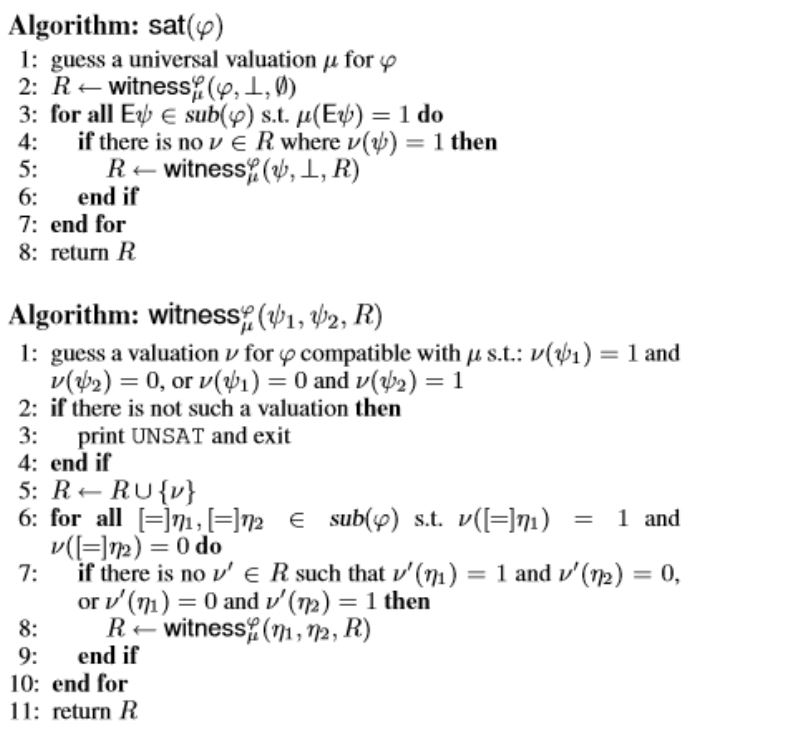
\includegraphics[height=\textheight]{satalgorithm.JPG}

\end{frame}

\begin{frame}
\Huge{\centerline{Preguntas??}}
\end{frame}

%----------------------------------------------------------------------------------------

\end{document}